\section{Algoritmo 1: Paralelismo de Datos con OpenMP}
\label{sec:algo1_omp}

\subsection{Implementación}
Se implementó en C++ el Algoritmo 1 aplicando paralelismo de datos mediante OpenMP sobre el bucle exterior de la multiplicación matricial densa de $N \times N$ ($N=2048$), utilizando la directiva \texttt{\#pragma omp parallel for schedule(static)}. De este modo, las $N$ filas de la matriz resultante $C$ se reparten de manera uniforme y determinista entre los $p$ hilos disponibles. Cada hilo calcula un bloque contiguo de filas independientes de $C$, accediendo a las filas correspondientes de $A$ y a la la matriz $B$ en su totalidad.

\begin{figure}[htbp]
    \centering
    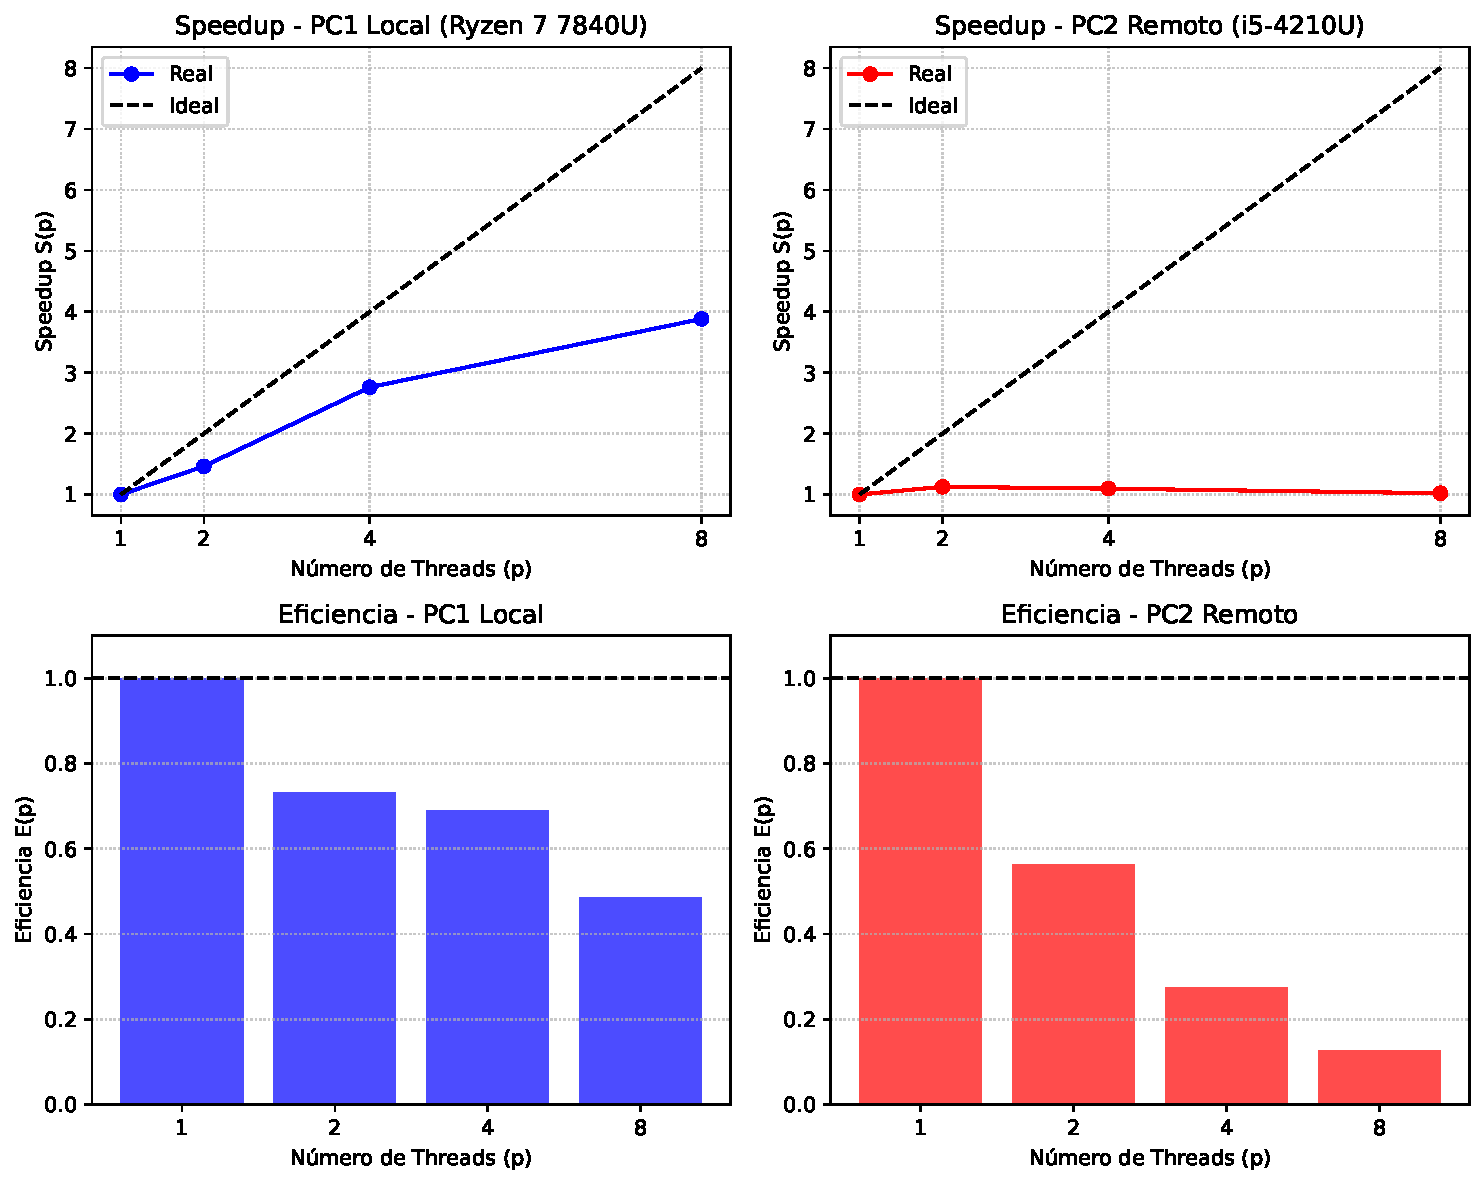
\includegraphics[width=\textwidth]{B/exp_b_plots.pdf}
    \caption{Resultados de Speedup y Eficiencia (Local vs. Remoto) para el Algoritmo 1 con OpenMP ($N=2048$).}
    \label{fig:exp_b_plots}
\end{figure}

\begin{table}[htbp]
\centering
\footnotesize
\setlength{\tabcolsep}{4pt}
\caption{Tiempos promedio (ms), Speedup $S(p)$ y Eficiencia $E(p)$ para el Algoritmo 1 ($N=2048$).}
\label{tab:resultados_b}
\begin{tabular}{r ccc ccc}
\toprule
& \multicolumn{3}{c}{\textbf{PC1 Local (AMD Ryzen 7 PRO 7840U)}} & \multicolumn{3}{c}{\textbf{PC2 Remoto (Intel Core i5-4210U)}} \\
\cmidrule(lr){2-4} \cmidrule(lr){5-7}
$p$ & Tiempo (ms) & Speedup $S(p)$ & Eficiencia $E(p)$ & Tiempo (ms) & Speedup $S(p)$ & Eficiencia $E(p)$ \\
\midrule
1 & 4579.82 & 1.0000 & 1.0000 & 6271.94 & 1.0000 & 1.0000 \\
2 & 3130.26 & 1.4631 & 0.7315 & 5569.35 & 1.1262 & 0.5631 \\
4 & 1658.09 & 2.7621 & 0.6905 & 5720.83 & 1.0963 & 0.2741 \\
8 & 1179.62 & 3.8824 & 0.4853 & 6143.11 & 1.0210 & 0.1276 \\
\bottomrule
\end{tabular}
\end{table}

\subsection{Análisis}
En \textbf{PC1 (AMD Ryzen 7 7840U)}, el algoritmo presenta un escalamiento sostenido hasta alcanzar un \emph{speedup} de $3.88\times$ con $p=8$ hilos. No obstante, la eficiencia decrece progresivamente desde $1.0$ hasta $0.485$. Esta degradación se atribuye principalmente a la saturación del ancho de banda de memoria (\emph{memory-bound}): en la estructura de bucles $i$-$k$-$j$, la matriz $B$ ($32$ MiB) es leída repetidamente por todos los hilos, sobrepasando la capacidad de la memoria caché L3 (16 MiB compartida) y generando un elevado tráfico hacia la memoria RAM principal, lo que causa contención entre los núcleos.

En \textbf{PC2 (Intel Core i5-4210U)}, el rendimiento se estanca tempranamente, alcanzando un \emph{speedup} máximo de apenas $1.13\times$ con $p=2$, e incluso empeorando con $p \ge 4$ ($1.02\times$ con $p=8$). Este comportamiento se explica por tres limitantes críticas de la arquitectura:
\begin{enumerate}
    \item \textbf{Recursos físicos limitados:} El procesador cuenta únicamente con 2 núcleos físicos reales (4 hilos lógicos vía Hyper-Threading). Con $p=4$ y $p=8$, múltiples hilos compiten por las mismas unidades de ejecución e introducen sobrecarga (\emph{overhead}) de cambio de contexto.
    \item \textbf{Estrangulamiento térmico y de potencia (\emph{throttling}):} Al operar bajo un TDP estricto de \SI{15}{\watt}, someter ambos núcleos al \SI{100}{\percent} de carga continua obliga al procesador a reducir drásticamente su frecuencia de reloj (\emph{downclocking}) con respecto a la frecuencia Turbo mononúcleo.
    \item \textbf{Capacidad de caché y latencia de memoria:} Con solo 3 MiB de caché L3 compartida, las matrices desbordan completamente la jerarquía de caché, convirtiendo el acceso a memoria en el cuello de botella dominante.
\end{enumerate}
